\section{Experimentación y rendimiento}
\subsection{Método y reproducibilidad}
Todos los experimentos leen el mismo CSV con \texttt{csv.DictReader} y lo convierten mediante el serializador del motor. Se conserva el orden ascendente de product\_id. La carga de índices B+ y Hash del experimento 1 incluye un Heap de productos completos y su índice; no se comparan únicamente pares clave/RID contra registros completos. Sus tiempos incluyen lectura del CSV, serialización y transferencias de archivos. No se incluye el Hash privado de unicidad del ejecutor en estas mediciones de estructuras aisladas.

Los experimentos 2 y 3 comparten un fixture persistente de 100\,000 productos. El Sequential se reorganiza a 75\% antes de las búsquedas. Los índices apuntan a los RID reales del Heap y se cuenta la recuperación del registro, no solo el acceso al índice. El experimento 4 aísla el árbol B+ y no recupera payloads; sus RID son etiquetas de prueba. Las claves de búsqueda se generan con semilla 42. La desviación estándar reportada es poblacional.

Las cifras provienen de operaciones reales, no de costos estimados. El SO mantiene su caché y la latencia depende del equipo y carga del sistema; pequeñas diferencias de tiempo entre índices no prueban superioridad general. La comparación de transferencias es más estable. Los resultados crudos, resúmenes CSV y gráficas se guardan en \texttt{benchmarks/results/} y \texttt{benchmarks/plots/}. Los experimentos se ejecutan secuencialmente entre sí.

\subsection{Validación del CSV después de reabrir}

\begin{table}[H]\centering\small
\caption{Importación integrada con comprobación de PRIMARY KEY. Creación de tabla medida por separado.}
\begin{tabular}{lrrrr}
\toprule
Filas & Verificadas & Tiempo (s) & Lecturas & Escrituras \\
\midrule
1\,000 & 1\,000 & 0.40 & 5\,934 & 4\,032 \\
10\,000 & 10\,000 & 4.79 & 64\,946 & 45\,944 \\
100\,000 & 100\,000 & 51.71 & 621\,088 & 431\,086 \\
500\,000 & 500\,000 & 323.00 & 3\,108\,130 & 2\,153\,577 \\
\bottomrule\end{tabular}\end{table}

La comparación recorre nuevamente el CSV y el Heap reabierto; exige igualdad de los bytes serializados de cada fila y comprueba los extremos del dominio. Los resultados completos incluyen lecturas/escrituras de creación en el JSON de validación.

\clearpage\subsection{Experimento 1: costo de inserción masiva}

\begin{table}[H]\centering\small
\caption{Tiempo de carga por estructura, en segundos.}
\begin{tabular}{lrrrrr}
\toprule
N & Heap & Seq. & Seq.+reorg. & Heap+B+ & Heap+Hash \\
\midrule
1\,000 & 0.04 & 0.05 & 0.06 & 0.21 & 0.30 \\
10\,000 & 0.38 & 0.55 & 0.60 & 2.48 & 3.64 \\
50\,000 & 1.90 & 2.70 & 2.95 & 14.72 & 17.75 \\
100\,000 & 3.84 & 5.39 & 5.92 & 30.42 & 36.80 \\
250\,000 & 9.52 & 13.44 & 14.90 & 78.22 & 102.69 \\
500\,000 & 19.11 & 26.96 & 29.72 & 161.69 & 213.45 \\
\bottomrule\end{tabular}\end{table}

\begin{table}[H]\centering\small
\caption{Escrituras reales de páginas por carga.}
\begin{tabular}{lrrrrr}
\toprule
N & Heap & Seq. & Seq.+reorg. & Heap+B+ & Heap+Hash \\
\midrule
1\,000 & 2\,001 & 2\,101 & 2\,246 & 3\,020 & 4\,037 \\
10\,000 & 20\,001 & 21\,001 & 22\,432 & 30\,198 & 45\,949 \\
50\,000 & 100\,001 & 105\,001 & 112\,146 & 150\,989 & 215\,297 \\
100\,000 & 200\,001 & 210\,001 & 224\,289 & 301\,979 & 431\,091 \\
250\,000 & 500\,001 & 525\,001 & 560\,718 & 754\,947 & 1\,080\,015 \\
500\,000 & 1\,000\,001 & 1\,050\,001 & 1\,121\,432 & 1\,509\,897 & 2\,153\,582 \\
\bottomrule\end{tabular}\end{table}

\begin{figure}[H]\centering
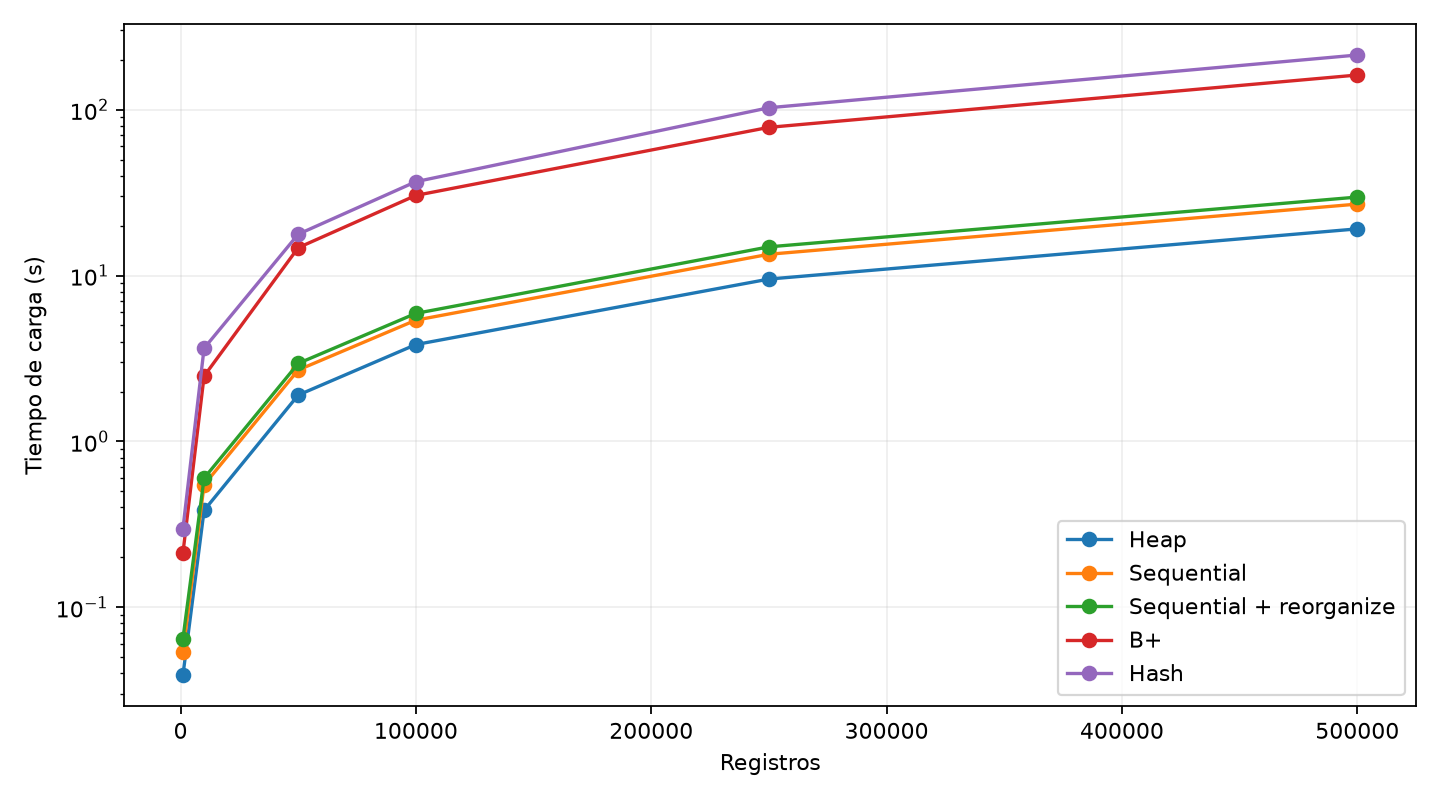
\includegraphics[width=.49\textwidth]{../benchmarks/plots/exp1_time.png}
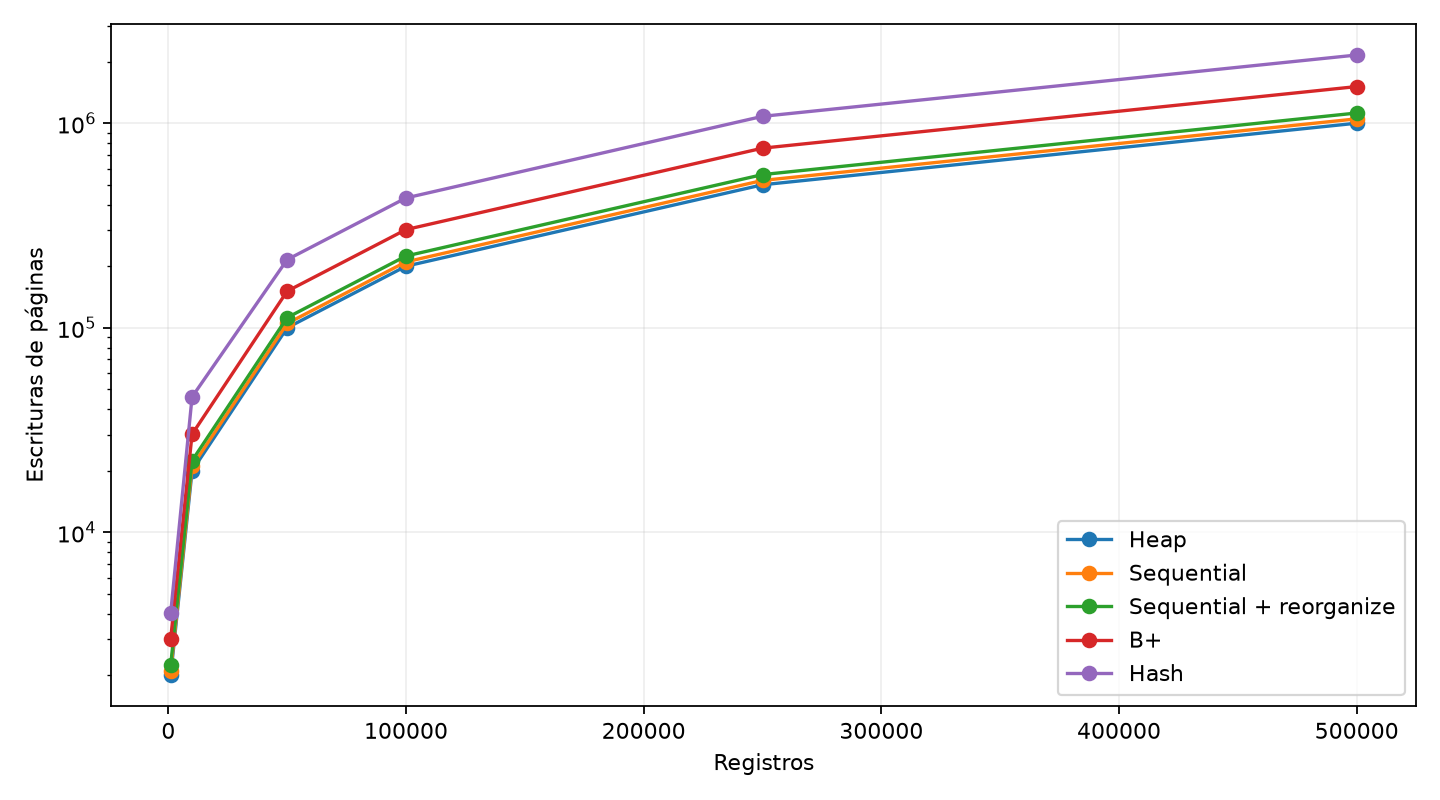
\includegraphics[width=.49\textwidth]{../benchmarks/plots/exp1_writes.png}
\caption{Cargas completas: tiempo y escrituras, con eje vertical logarítmico.}\end{figure}

Heap escribe la página del registro y su metadata en cada inserción. Sequential aprovecha el CSV ascendente; reorganizar añade la lectura del principal y su reescritura con espacios libres. B+ y Hash incorporan mantenimiento del índice además del payload. La cantidad de escrituras incluye inicialización y splits reales. Este workload no mide el peor caso de overflow desordenado.

\clearpage\subsection{Experimento 2: igualdad}

\begin{table}[H]\centering\small
\caption{1000 consultas de igualdad sobre 100000 productos; incluye recuperar la fila.}
\begin{tabular}{lrrrr}
\toprule
Estructura & Media I/O & Desv. I/O & Media ms & Desv. ms \\
\midrule
Heap & 10\,000.000 & 0.000 & 161.0724 & 3.4962 \\
Sequential & 14.971 & 0.508 & 0.1910 & 0.0352 \\
B+ & 4.022 & 0.147 & 0.1515 & 0.0335 \\
Hash & 3.000 & 0.000 & 0.1614 & 0.0331 \\
\bottomrule\end{tabular}\end{table}

\begin{figure}[H]\centering
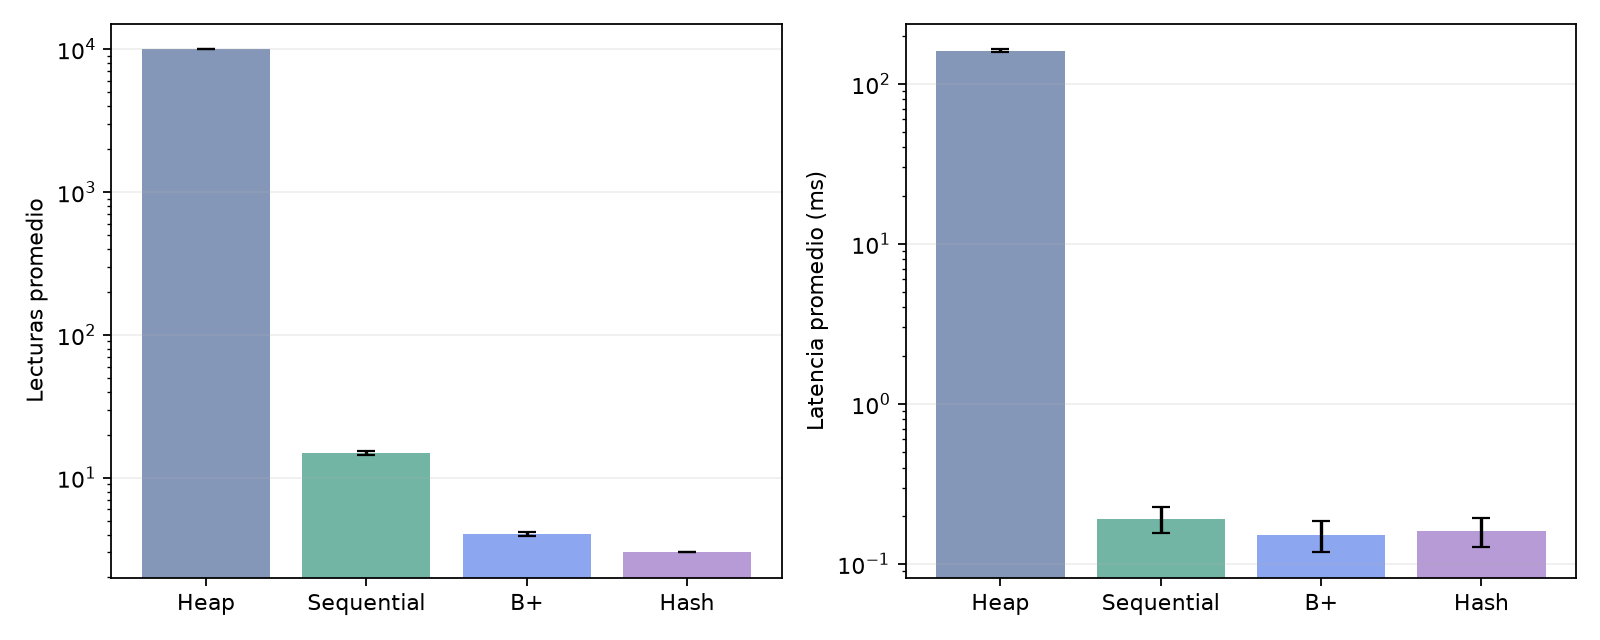
\includegraphics[width=.94\textwidth]{../benchmarks/plots/exp2_point.png}
\caption{Media y desviación estándar poblacional; escala logarítmica.}\end{figure}

El Full Scan lee las 10000 páginas de productos en cada consulta. Sequential necesita la búsqueda binaria y la página candidata. El B+ desciende desde la raíz y recupera el payload del Heap; algunas consultas leen una hoja adicional para cerrar el rango de igualdad. Hash lee una página del directorio, un bucket y una página de datos. La desviación nula de I/O del Hash observado indica ausencia de cadenas para estas claves únicas; no es una garantía para cualquier distribución.

\clearpage\subsection{Experimento 3: selectividad de rangos}

\begin{table}[H]\centering\small
\caption{Rangos inclusivos centrados en el dominio; cardinalidad verificada en cada consulta.}
\begin{tabular}{lrrrrrr}
\toprule
Sel. (\%) & Heap I/O & Seq. I/O & B+ I/O & Heap ms & Seq. ms & B+ ms \\
\midrule
0.1 & 10\,000 & 28 & 15 & 163.05 & 0.47 & 0.97 \\
1.0 & 10\,000 & 158 & 114 & 160.82 & 2.71 & 2.11 \\
5.0 & 10\,000 & 728 & 553 & 160.26 & 12.44 & 9.77 \\
10.0 & 10\,000 & 1\,444 & 1\,102 & 162.85 & 26.20 & 20.26 \\
25.0 & 10\,000 & 3\,586 & 2\,749 & 163.15 & 63.29 & 50.78 \\
\bottomrule\end{tabular}\end{table}

\begin{figure}[H]\centering
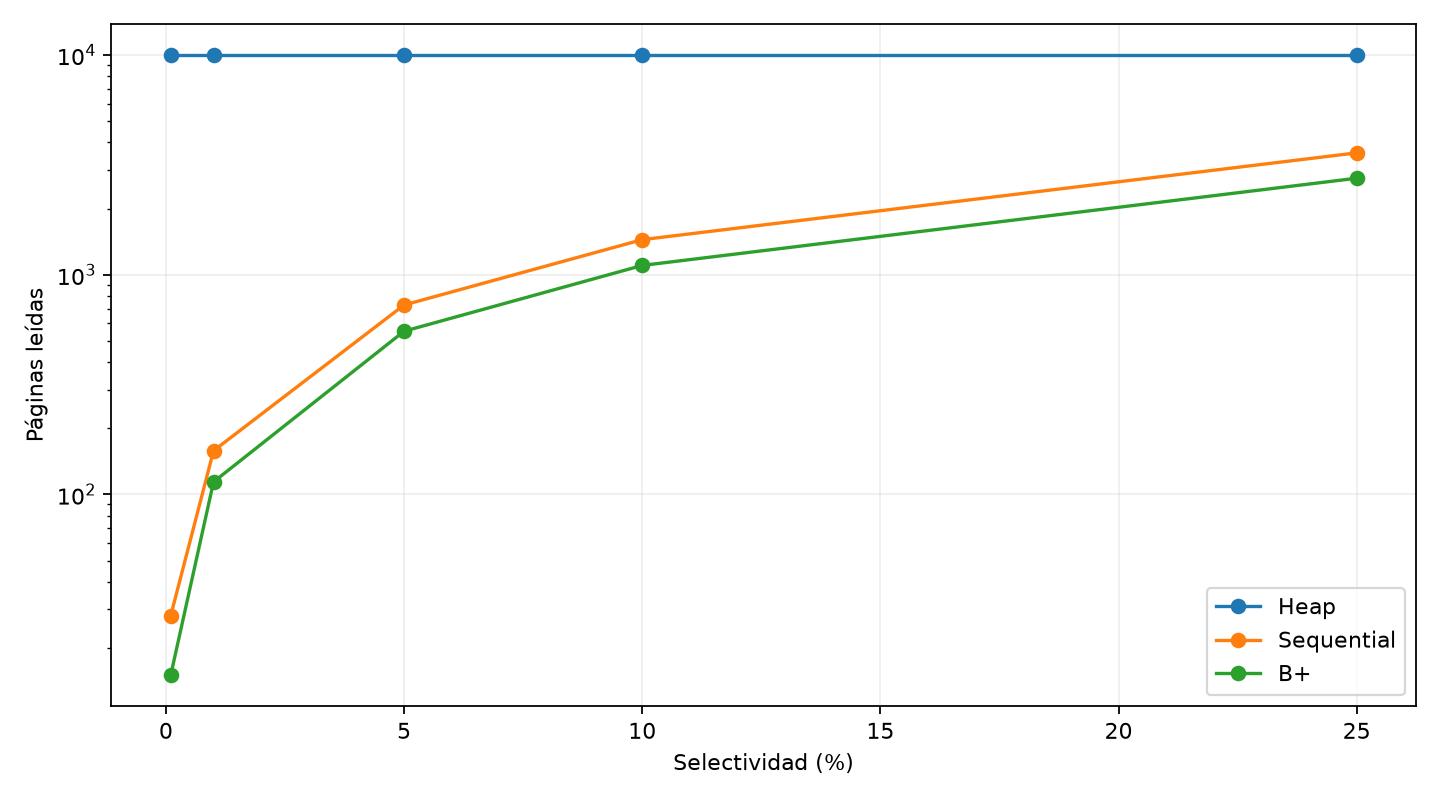
\includegraphics[width=.49\textwidth]{../benchmarks/plots/exp3_reads.png}
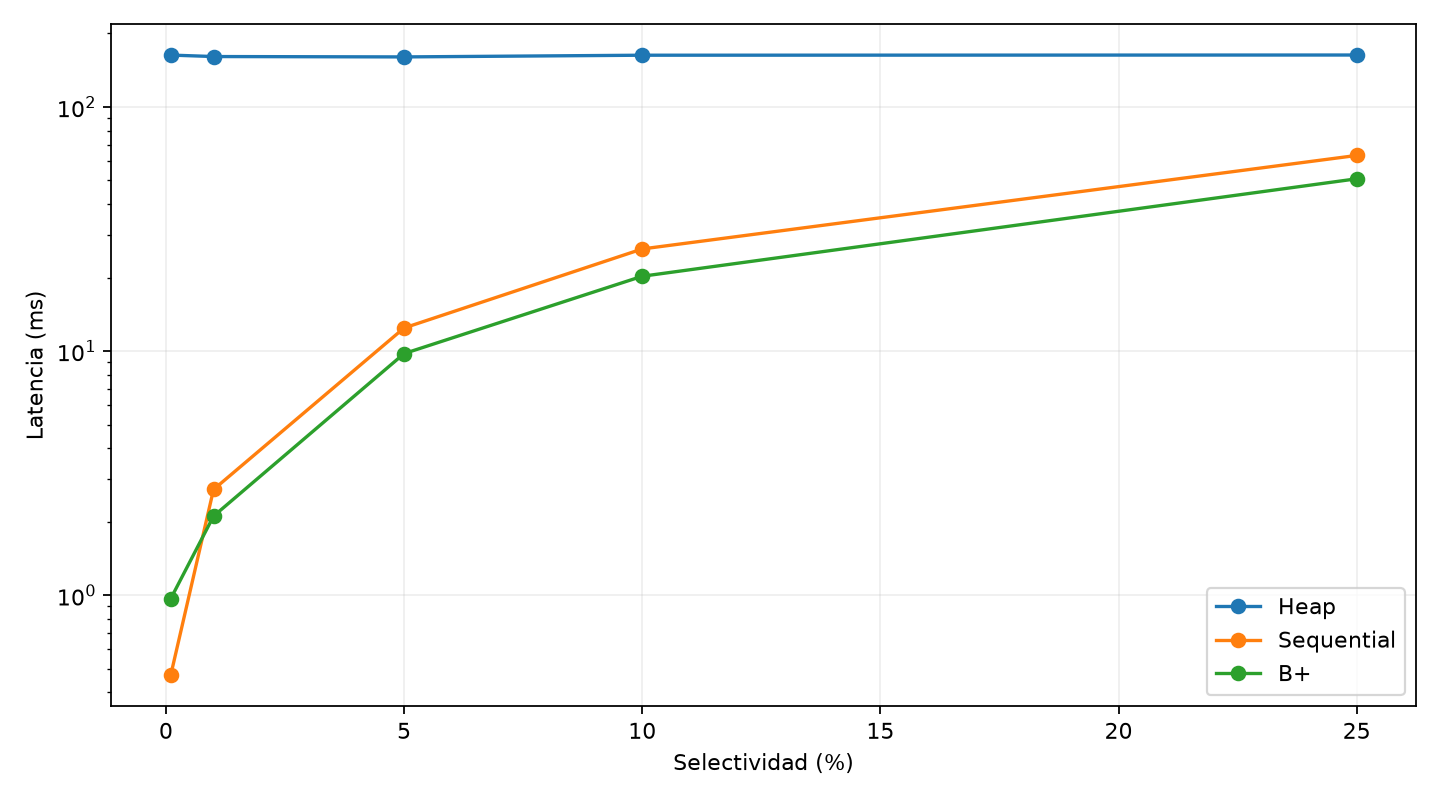
\includegraphics[width=.49\textwidth]{../benchmarks/plots/exp3_time.png}
\caption{Costo de rangos según selectividad, con escala vertical logarítmica.}\end{figure}

Heap mantiene un costo de escaneo completo independientemente de cuántas filas satisfacen el predicado. Sequential y B+ incrementan sus lecturas a medida que el rango necesita más páginas. El Sequential reorganizado contiene siete productos por página, mientras el Heap de payloads del B+ contiene diez; parte de la diferencia procede de esta ocupación, además del costo de navegar el índice. Las consultas del B+ reutilizan una página de datos durante la recuperación de RID consecutivos.

\clearpage\subsection{Experimento 4: sensibilidad al tamaño de página}

\begin{table}[H]\centering\small
\caption{Árbol B+ con 100000 claves; 1000 búsquedas. No incluye recuperar productos.}
\begin{tabular}{lrrrrr}
\toprule
Bytes & Fan-out & Altura & Páginas & I/O búsqueda & Escrituras carga \\
\midrule
1\,024 & 50 & 4 & 4\,160 & 4.071 & 108\,315 \\
2\,048 & 102 & 3 & 1\,999 & 3.039 & 103\,994 \\
4\,096 & 204 & 3 & 991 & 3.022 & 101\,978 \\
8\,192 & 409 & 3 & 494 & 3.012 & 100\,984 \\
\bottomrule\end{tabular}\end{table}

\begin{figure}[H]\centering
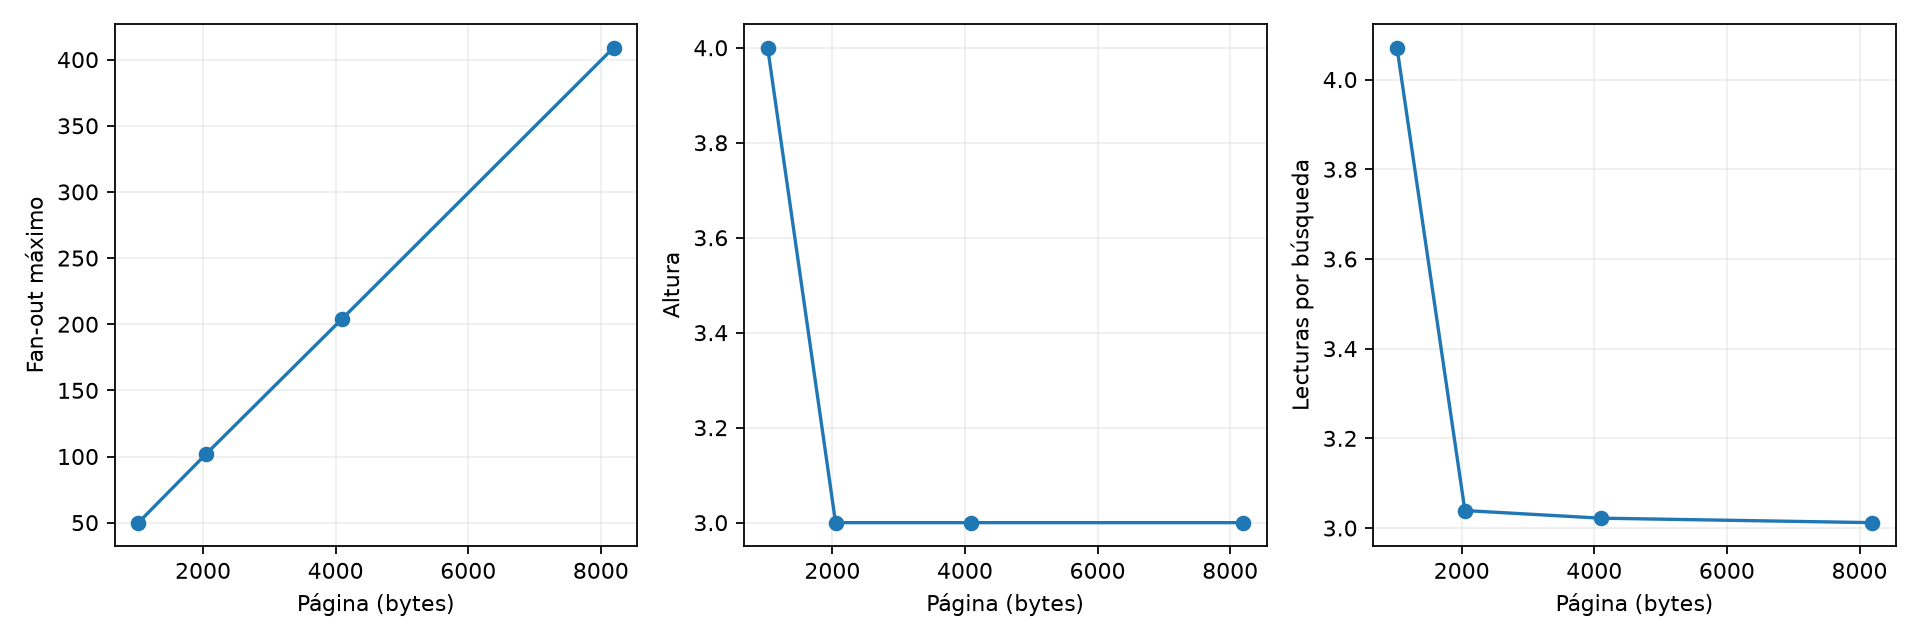
\includegraphics[width=.94\textwidth]{../benchmarks/plots/exp4_page_size.png}
\caption{Estructura y lecturas del B+ para los cuatro tamaños de página.}\end{figure}

Con 1024 bytes, el árbol requiere cuatro niveles; con los tamaños mayores, tres. Aumentar la capacidad reduce el número de nodos y las escrituras de splits. La latencia de construcción no disminuye necesariamente: el serializador procesa más entradas por nodo al aumentar el tamaño de página. La reducción de I/O debe distinguirse del costo de CPU y de la caché del SO.

